\subsection{\textbf{\uppercase{Implementação do Middleware}}}

O \textit{Middleware} intermediário denominado Integrador será responsável em receber as solicitações realizadas pela URA do Asterisk, após analisá-las deverá efetuar requisições ao \textit{WebService} do sistema GSAN, a fim de obter as informações, logo em seguida tratá-las e então devolver as informações essenciais ao Asterisk.
O \textit{Middleware} é capaz de comunicar-se com os sistemas GSAN e Asterisk. A comunicação com o sistema GSAN é realizada por uma implementação cliente do \textit{Webservice} disponibilizado, já a comunicação com o Asterisk é realizada por uma interface de comunicação chamada AGI, neste trabalho foi utilizado o \textit{framework} \textit{Open Source} chamado Asterisk-Java, que fornece recursos para comunicação com o Asterisk utilizando os protocolos comuns ao sistema.

Para cada novo serviço a ser tratado pelo Middleware, é necessário declarar uma chave de texto que será utilizada no Asterisk, que representa o objeto a ser invocado, adicionados em um novo arquivo chamado \textit{fastagi-mapping.properties} da seguinte maneira, conforme a figura \ref{figura:mapeamenteServicosAGI} abaixo:

\begin{figure}[H]
	\centering
	\caption{\textbf{Mapeamento dos serviços para consumo via AGI}}
	\label{figura:mapeamenteServicosAGI}
	\begin{subfigure}[H]{\textwidth}
		\centering
		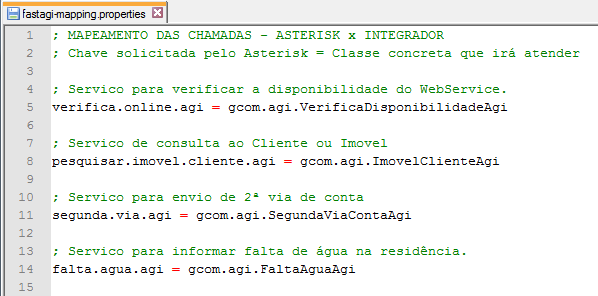
\includegraphics{figuras/mapeamento_servicos_agi.png}
		\legend {\fontsize{10}{12}\selectfont {Fonte: Autoria Própria}.}	
	\end{subfigure}
\end{figure}



Dessa forma o \textit{Middleware} tem condições de recepcionar as solicitações originadas pelo \textit{software} Asterisk utilizando a interface de comunicação AGI, e direcionar a chamada internamente para uma classe concreta que contém a lógica de consumo aos novos serviços disponibilizados pelo \textit{WebService} do sistema GSAN.

Para cada classe concreta a ser disponibilizada é necessário estender a classe \textit{BaseAgiScript} disponibilizada pelo \textit{framework} Asterisk-Java, em seguida é preciso implementar o método \textit{service} obtido pela herança da \textit{BaseAgiScript}, tal método será invocado quando a requisição for direcionada ao serviço mapeado no arquivo \textit{fastagi-mapping.properties}, segue abaixo um exemplo de implementação utilizado, conforme a figura \ref{figura:fluxoIdentificacaoCliente} abaixo:

% Custom exibição da lista de algoritmos
%\algsetup{
%	linenosize=\small,
%	linenodelimiter=.	
%}

%\begin{algorithm}
%	\caption{Novo serviço de identificação do cliente (\textit{Middleware}).}	
%	\label{algoritmo:identificaoCliente}
%	\begin{algorithmic}[1]
%		\STATE $atenderLigação()$ 		
%		\COMMENT{Recepciona a liga}
%		\STATE $digitoInformado \gets canal[cliente]$ 	\COMMENT{Obtém os dígitos informados}
%		\IF{ $valorInformado <> null$ }
%		\STATE $ws \gets obterWebService() $ 
%		\COMMENT{Obtém a instância do WebService}
%		\STATE $retorno \gets ws.pesquisarImovelOuCliente(valorInformado) $
%		\COMMENT{Realiza a requisição}
%		\STATE $ tratarRetorno(retorno) $
%		\COMMENT{Verifica o retorno obtido}
%		\ELSE		
%		\STATE $ tocarAudio(informar\_valor) $
%		\COMMENT{Tocar o áudio de aviso}
%		\STATE $ canal[situacao] \leftarrow erro $
%		\COMMENT{Sinaliza o erro}
%		\ENDIF		
%	\end{algorithmic}
%\end{algorithm}

\begin{figure}[H]
	%\centering
	\caption{\textbf{Fluxo de Identificação de Cliente no Middleware.}}	
	\label{figura:fluxoIdentificacaoCliente}
	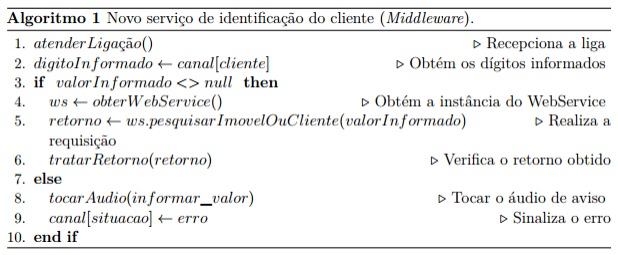
\includegraphics{figuras/algoritmo_1.png}
	\\[6pt]
	\fontsize{10}{12}\selectfont {Fonte: Autoria Própria.}
\end{figure}
%	\legend{\fontsize{10}{12}\selectfont {Fonte: Autoria Própria.}}

Visando facilitar o consumo dos novos serviços, será gerado o \textit{WebService} cliente a partir do WSDL\footnote{WSDL - \textit{Web Services Description Language}} da interface do serviço disponibilizada no sistema GSAN, utilizando o software chamado WSIMPORT disponibilizado pela \textit{Sun Microsystems}, conforme visto na figura \ref{figura:gerarWSCliente}:

\begin{figure}[H]
	\centering
	\caption{\textbf{Geração do código fonte para consumo do WebService.}}	
	\label{figura:gerarWSCliente}
	\begin{subfigure}[H]{\textwidth}
		\centering
		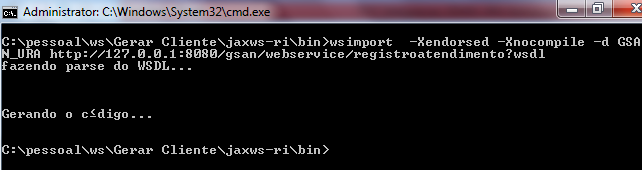
\includegraphics{figuras/gerar_wscliente.png}
		\legend {\fontsize{10}{12}\selectfont {Fonte: Autoria Própria}.}	
	\end{subfigure}
\end{figure}

Descrição dos parâmetros utilizados:

\begin{description}
	\item \textbf{\textit{–Xendorsed}}: Necessário para realizar a substituição dos padrões endossados do sistema, ou seja, utiliza a versão correta da JDK para realizar o \textit{parser}.
	\item \textbf{\textit{–Xnocompile}}: Utilizado para gerar o código fonte não compilado, ou seja, o arquivo na extensão .java.
	\item \textbf{\textit{-d}}: Informado para determinar o diretório para onde os arquivos devem ser gerados, no exemplo o diretório se chama "GSAN\_URA".
	\item Por último a URL que disponibiliza o WSDL dos serviços. 
\end{description}



Com isso será gerado o código fonte de consumo dos serviços atualmente declarados na interface do \textit{EndPoint}, para cada modificação na interface será necessário realizar o procedimento novamente. O \textit{Middleware} deve ser disponibilizado em um terminal, que seja acessível ao Asterisk, para que o mesmo consiga realizar requisições aos objetos mapeados anteriormente, neste trabalho o \textit{Middleware} foi executado no mesmo hospedeiro do Asterisk, conforme visto na figura \ref{figura:executarIntegrador} abaixo:

\begin{figure}[H]
	\centering
	\caption{\textbf{Executando o sistema Integrador.}}	
	\label{figura:executarIntegrador}
	\begin{subfigure}[H]{\textwidth}
		\centering
		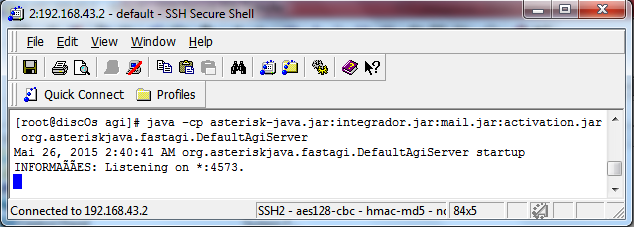
\includegraphics{figuras/executar_integrador.png}
		\legend {\fontsize{10}{12}\selectfont {Fonte: Autoria Própria}.}	
	\end{subfigure}
\end{figure}


A instrução realizada acima executa a classe principal do \textit{framework} Asterisk-Java a \textit{ org.asteriskjava.fastagi.DefaultAgiServer}, inicializando o serviço de comunicação via AGI, sob a JVM\footnote{JVM - \textit{Java Virtual Machine}} da plataforma Java, passando como \textit{Classpath}\footnote{Classpath refere-se a uma variável de ambiente que indica o local onde as dependências estão localizadas.} as seguintes bibliotecas: 
%Citar classpath - pendente

\begin{itemize}
	\item \textbf{\textit{asterisk-java.jar}}: biblioteca do \textit{framework} utilizado para se comunicar com o Asterisk.
	\item \textbf{\textit{integrador.jar}}: o \textit{Middleware} que integra as aplicações.
	\item \textbf{\textit{mail.jar}} e \textbf{\textit{activation.jar}}: ambos necessários no envio de e-mail, para os casos de Obter 2ª via de conta.	
\end{itemize}

Após estes passos o sistema Integrador já estará apto a receber solicitações do Asterisk e realizar requisições para o Sistema GSAN.